\documentclass[a4paper]{article}
\usepackage[pdftex]{graphicx}
\usepackage[utf8]{inputenc}
\usepackage{enumerate}
\usepackage{siunitx}
\sisetup{locale=DE} 
\usepackage{icomma}
\usepackage{amssymb}
\usepackage{tikz}
\usepackage{href-ul}
\hypersetup{
	colorlinks=true,
	linkcolor=blue,
	urlcolor=blue}
\usepackage{geometry}
\geometry{a4paper, top=15mm, left=15mm, right=15mm, bottom=15mm,
	headsep=10mm, footskip=12mm}

\begin{document}
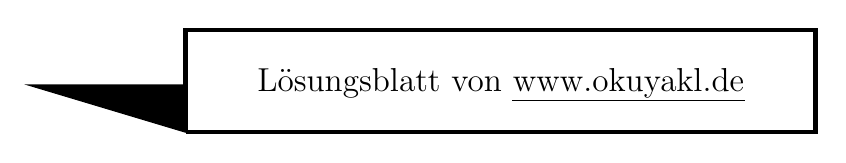
\begin{tikzpicture}(10,3)
	\draw[ultra thick](2,0) --(10,0) -- (10,1.3) --(2,1.3) -- (2,0);
	\draw[fill=black](2,0)-- (0,.6) -- (2,.6) -- (2,0);
	\node at (6,.6) {\large Lösungsblatt von \href{https://www.okuyakl.de}{www.okuyakl.de}};
\end{tikzpicture}
\vspace{0.5 cm}

\noindent{\bf Aufgabe 1. a)}\\
Nur Dauermagneten werden gefärbt - üblicherweise ist bei diesen der Nordpol rot und der Südpol grün. Bei einem Elektromagneten kann man die Polung mit einer Kompassnadel überprüfen. Deren Nordspitze zeigt dann zum Südpol.

\noindent{\bf Aufgabe 1. b)}\\
In einem unverzweigten Stromkreis ist die Stromstärke überall gleich, also leuchten beide Lampen gleich hell.

\noindent{\bf Aufgabe 2. a)}\\
Beide Stäbe werden gleichsinnig magnetisiert. Dabei ziehen sich der Südpol des einen Stabes und der Nordpol des anderen Stabes an. Die Stäbe haften aneinander.

\noindent{\bf Aufgabe 2 b)}\\
Beide Stäbe werden wieder gleichsinnig magnetisiert. Nun liegen aber gleiche Pole nebeneinander. Die Stäbe stoßen sich ab.


\noindent
\begin{minipage}{0.5\textwidth}
	\noindent{\bf Aufgabe 3. a)}\\
	\includegraphics[width=5 cm]{stro403}
\end{minipage}
\hfill
\begin{minipage}{0.5\textwidth}
	\noindent{\bf Aufgabe 3. b)}\\
	\includegraphics[width=5 cm]{span403}
\end{minipage}

\noindent
\begin{minipage}{0.3\textwidth}
	\noindent{\bf Aufgabe 4. a)}\\
	\includegraphics[width=4 cm]{zwgl403}
\end{minipage}
\hfill
\begin{minipage}{0.3\textwidth}
	\noindent{\bf Aufgabe 4. b)}\\
	Durch beide Glühbirnen fließt der gleiche Strom.
	\includegraphics[width=4 cm]{zwi403}
\end{minipage}
\hfill
\begin{minipage}{0.3\textwidth}
	\noindent{\bf Aufgabe 4. c)}\\
	\includegraphics[width=4 cm]{zwu403}
\end{minipage}

\noindent{\bf Aufgabe 5. a)}\\
Die in diesem Akku gespeicherte Energie beträgt:
$$ E_{el} = \SI{12}{\volt}\cdot \SI{3,0}{\ampere\hour} =\SI{36}{\watt\hour}$$
Die Betriebsdauer ist damit:
$$ P = {E_{el} \over t} \quad \Rightarrow \quad t = {E_{el} \over P} = {\SI{36}{\watt\hour} \over \SI{24}{\watt}} =
\SI{1,5}{\hour}$$

\noindent{\bf Aufgabe 5. b)}\\
$$
\renewcommand{\arraystretch}{2}
\begin{array}{rcll}
E_{pot} &=& m\cdot g \cdot h = E_{el} &|:m \quad |:g\\
{E_{el} \over  m\cdot g } & = & h \\
h & = & {24\cdot \SI{3600}{\watt\second} \over \SI{105}{\kilogram} \cdot \SI{9,81}{\meter\over {\second^2}}}\\
h & = & \SI{83}{\meter}
\end{array}
$$

\begin{center}
	\includegraphics[width=7 cm]{../../viecher/endcomic.pdf}
	
	Hier geht es zurück zum \href{https://www.okuyakl.de/phys/p9eleL403/aa403.pdf}{Aufgabenblatt}
\end{center}


\end{document}


